\documentclass[tikz,border=4pt]{standalone}
\usepackage{amsmath}
\begin{document}
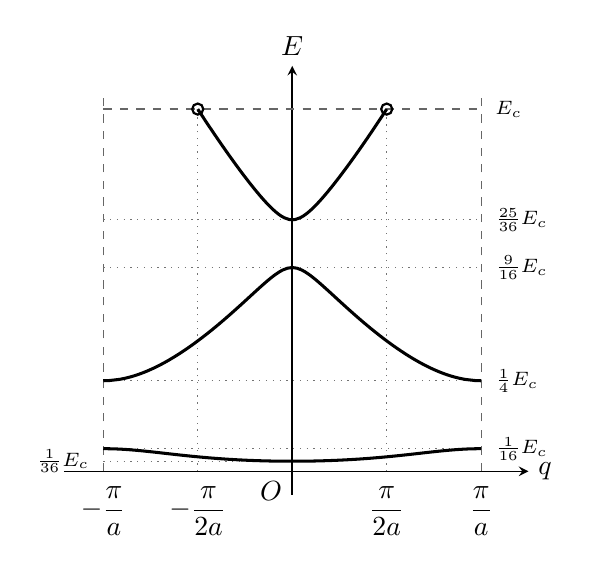
\begin{tikzpicture}[>=stealth, thick, scale=1.0]
  % Reduced-zone dispersion relation E(q) for kc*a - c = 5*pi/2
  % Horizontal: x = 2.4 * (q*a / pi)  =>  x in [-2.4, 2.4]
  % Vertical:   y = 4.6 * (E / Ec) = 4.6 * u^2  =>  y in [0, 4.6]
  % Band 1: u in [1/6, 1/4],  E/Ec in [1/36, 1/16] = [0.0278, 0.0625] -> y in [0.128, 0.288]
  % Band 2: u in [1/2, 3/4],  E/Ec in [1/4, 9/16]  = [0.25, 0.5625]   -> y in [1.150, 2.588]
  % Band 3: u in [5/6, 1),    E/Ec in [25/36, 1)   = [0.6944, 1)      -> y in [3.194, 4.600]

  % Axes
  \draw[->, line width=0.55pt] (-2.9, 0) -- (3.0, 0) node[right] {$q$};
  \draw[->, line width=0.55pt] (0, -0.3) -- (0, 5.15) node[above] {$E$};
  \node[below left] at (0, 0) {$O$};

  % Brillouin zone boundaries q = +/- pi/a
  \draw[dashed, line width=0.5pt, black!60] (-2.4, 0) -- (-2.4, 4.8);
  \draw[dashed, line width=0.5pt, black!60] (2.4, 0) -- (2.4, 4.8);
  \node[below] at (-2.4, -0.06) {$-\dfrac{\pi}{a}$};
  \node[below] at (2.4, -0.06) {$\dfrac{\pi}{a}$};

  % Half-zone ticks q = +/- pi/(2a)
  \draw[dotted, line width=0.45pt, black!55] (-1.2, 0) -- (-1.2, 4.6);
  \draw[dotted, line width=0.45pt, black!55] (1.2, 0) -- (1.2, 4.6);
  \node[below] at (-1.2, -0.06) {$-\dfrac{\pi}{2a}$};
  \node[below] at (1.2, -0.06) {$\dfrac{\pi}{2a}$};

  % Reference horizontal dotted lines for band edges
  \draw[dotted, line width=0.45pt, black!55] (-2.4, 0.128) -- (0.0, 0.128);
  \draw[dotted, line width=0.45pt, black!55] (-2.4, 0.288) -- (2.4, 0.288);
  \draw[dotted, line width=0.45pt, black!55] (-2.4, 1.150) -- (2.4, 1.150);
  \draw[dotted, line width=0.45pt, black!55] (-2.4, 2.588) -- (2.4, 2.588);
  \draw[dotted, line width=0.45pt, black!55] (-2.4, 3.194) -- (2.4, 3.194);
  \draw[dashed, line width=0.5pt, black!60] (-2.4, 4.600) -- (2.4, 4.600);

  % Band 1: u in [1/6, 1/4]
  \draw[line width=1.1pt] (0, 0.128) -- plot[domain=0.1670:0.2495, samples=60]
    ({2.4*acos(cos(450*\x)/sin(90*\x))/180}, {4.6*\x*\x}) -- (2.4, 0.288);
  \draw[line width=1.1pt] (0, 0.128) -- plot[domain=0.1670:0.2495, samples=60]
    ({-2.4*acos(cos(450*\x)/sin(90*\x))/180}, {4.6*\x*\x}) -- (-2.4, 0.288);

  % Band 2: u in [1/2, 3/4]
  \draw[line width=1.1pt] (2.4, 1.150) -- plot[domain=0.5005:0.7495, samples=80]
    ({2.4*acos(cos(450*\x)/sin(90*\x))/180}, {4.6*\x*\x}) -- (0, 2.588);
  \draw[line width=1.1pt] (-2.4, 1.150) -- plot[domain=0.5005:0.7495, samples=80]
    ({-2.4*acos(cos(450*\x)/sin(90*\x))/180}, {4.6*\x*\x}) -- (0, 2.588);

  % Band 3: u in [5/6, 1)
  \draw[line width=1.1pt] (0, 3.194) -- plot[domain=0.8338:0.9995, samples=60]
    ({2.4*acos(cos(450*\x)/sin(90*\x))/180}, {4.6*\x*\x}) -- (1.2, 4.600);
  \draw[line width=1.1pt] (0, 3.194) -- plot[domain=0.8338:0.9995, samples=60]
    ({-2.4*acos(cos(450*\x)/sin(90*\x))/180}, {4.6*\x*\x}) -- (-1.2, 4.600);

  % Open circles at upper limit E = Ec (k < kc)
  \draw[line width=0.8pt] (1.2, 4.6) circle (2.0pt);
  \draw[line width=0.8pt] (-1.2, 4.6) circle (2.0pt);

  % Energy labels
  \node[left, font=\scriptsize] at (-2.45, 0.128) {$\frac{1}{36}E_c$};
  \node[right, font=\scriptsize] at (2.45, 0.288) {$\frac{1}{16}E_c$};
  \node[right, font=\scriptsize] at (2.45, 1.150) {$\frac{1}{4}E_c$};
  \node[right, font=\scriptsize] at (2.45, 2.588) {$\frac{9}{16}E_c$};
  \node[right, font=\scriptsize] at (2.45, 3.194) {$\frac{25}{36}E_c$};
  \node[right, font=\scriptsize] at (2.45, 4.600) {$E_c$};
\end{tikzpicture}
\end{document}
